\Problem
{معماری شبکه‌های سلولی}
{
از منظر اهراز اصالت، یک شبکه سلولی از سه مولفه اصلی تشکیل شده است.
این مولفه‌ها در شکل زیر نمایش داده شده اند.

\begin{figure}[H]
    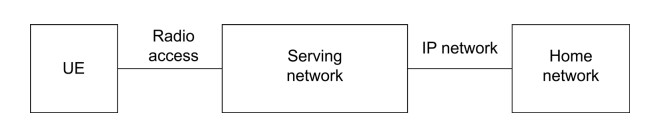
\includegraphics[width=15cm]{Images/IMG_02.jpg}
    \centering
    \caption{معماری شبکه‌های سلولی}
\end{figure}

\lr{UE}
همان سیمکارت می‌باشد که المان
\lr{UICC}
را شامل می‌شود.
این المان کلیدهای رمزنگاری را درون خود ذخیره دارد. این کلیدها با کلیدهای سمت شبکه یکی است.

\lr{Serving Network}
در واقع همان
\lr{RAN}
می‌باشد که شامل تجهیزات دسترسی هوایی است.
\lr{eNodeB} و \lr{MME}
اسامی آشنایی هستند که در کلاس درس مورد بررسی قرار گرفتند.

\lr{Home Network}
در واقع مانند هسته شبکه هست که شامل سرورهای اهراز اصالت است.
برای مثال
\lr{Home Subscriber Server (HSS)}
گواهینامه کاربرهای اهراز اصالت شده را نگه می‌دارد.

ارتباط میان
\lr{Serving Network} و \lr{Home Network}
از طریق
\lr{IP}
برقرار است.

ماهیت‌های اصلی که تحت
\lr{IP}
به هم متصل هستتند معمولا تحت عنوان
\lr{Evolved Packet System (EPS)}
شناخته می‌شوند.
}
